\section{Referencia de la Clase Sub\-Form2Bf}
\label{classSubForm2Bf}\index{SubForm2Bf@{SubForm2Bf}}
Clase Sub\-Form2Bf.  


{\tt \#include $<$subform2bf.h$>$}

Diagrama de herencias de Sub\-Form2Bf\begin{figure}[H]
\begin{center}
\leavevmode
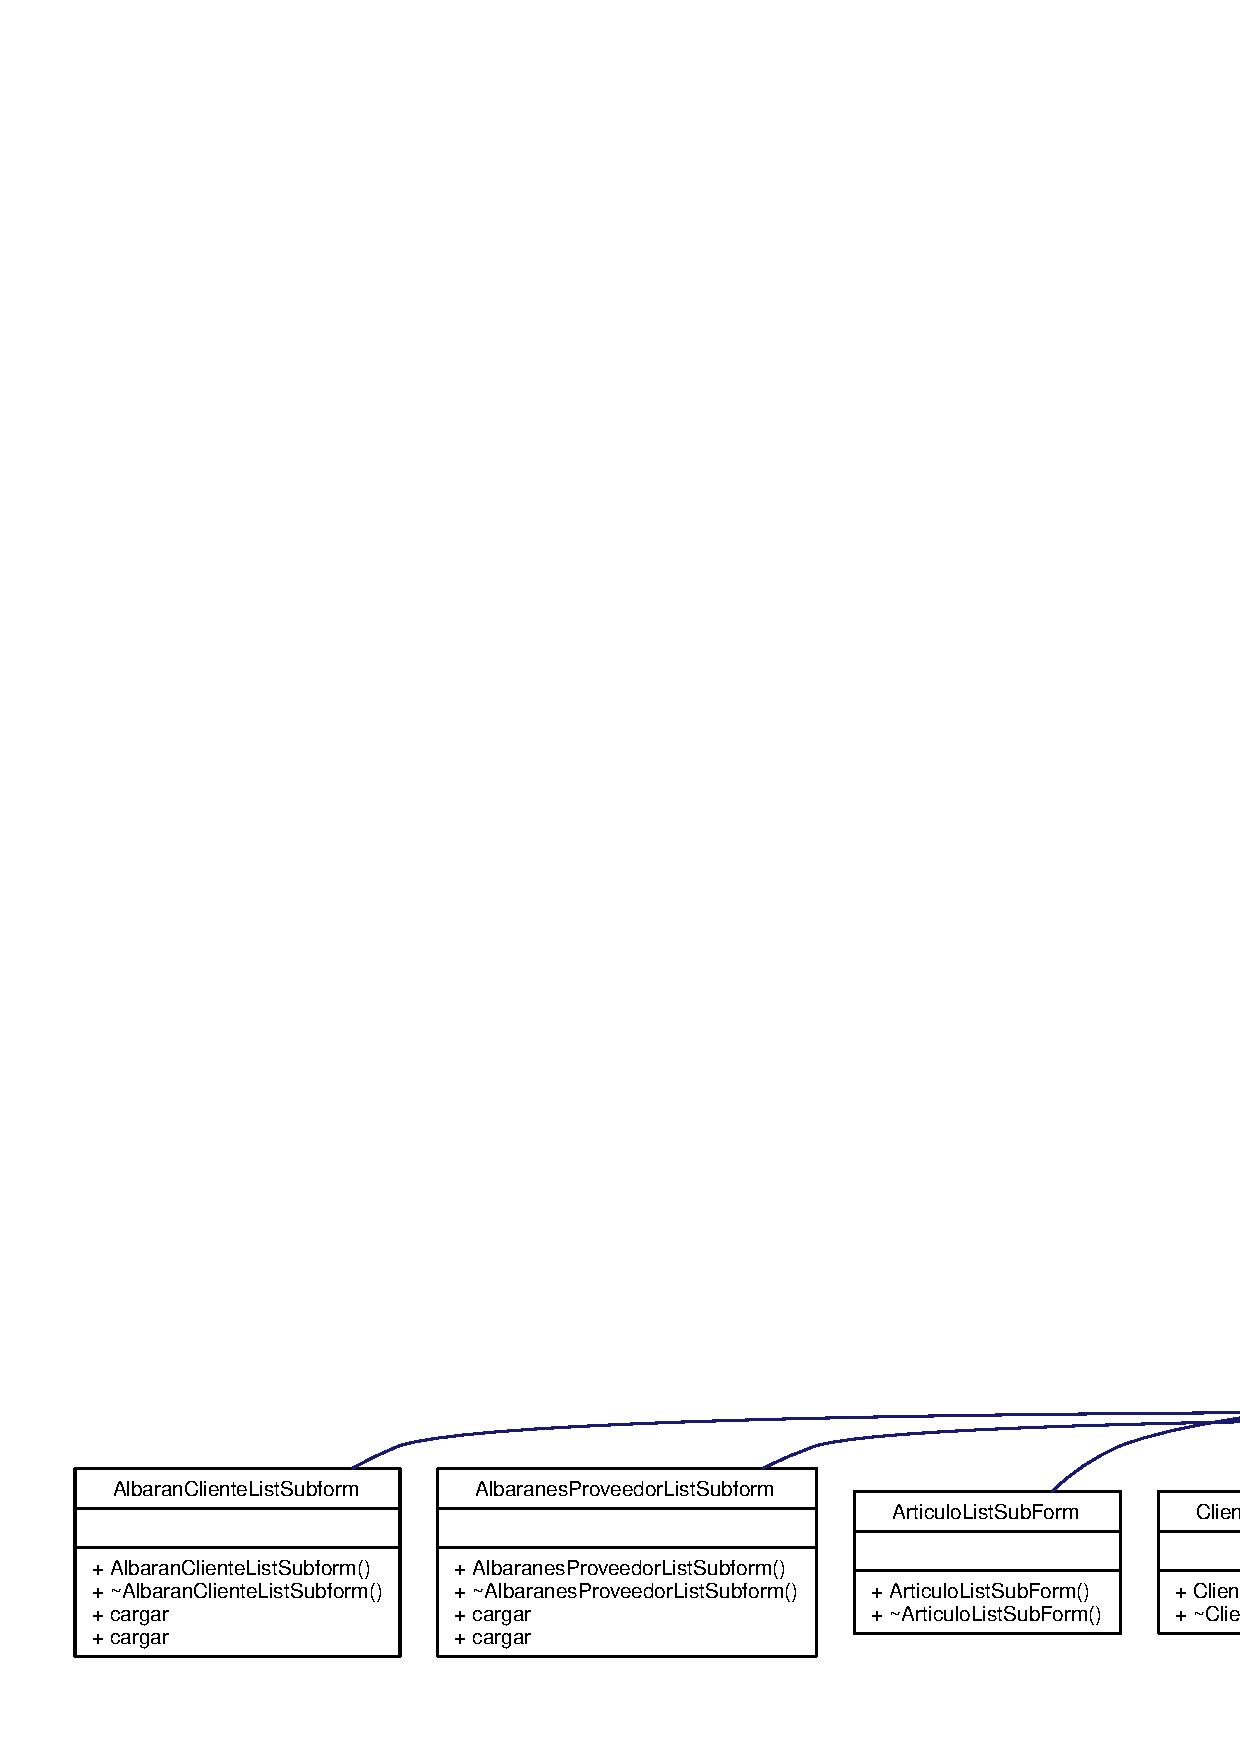
\includegraphics[width=420pt]{classSubForm2Bf__inherit__graph}
\end{center}
\end{figure}
\subsection*{Slots p\'{u}blicos}
\begin{CompactItemize}
\item 
virtual void {\bf context\-Menu\-Event} (QContext\-Menu\-Event $\ast$)\label{classSubForm2Bf_i0}

\item 
virtual void {\bf on\_\-mui\_\-list\_\-edit\-Finished} (int row, int col)\label{classSubForm2Bf_i1}

\item 
virtual void {\bf on\_\-mui\_\-list\_\-pressed\-Asterisk} (int row, int col)
\item 
virtual void {\bf on\_\-mui\_\-list\_\-pressed\-Minus} (int row, int col)
\item 
virtual void {\bf on\_\-mui\_\-list\_\-pressed\-Slash} (int row, int col)\label{classSubForm2Bf_i4}

\end{CompactItemize}
\subsection*{M\'{e}todos p\'{u}blicos}
\begin{CompactItemize}
\item 
virtual void {\bf cargar} (QString query)\label{classSubForm2Bf_a0}

\item 
void {\bf set\-Delete} (bool f)\label{classSubForm2Bf_a1}

\item 
{\bf Sub\-Form2Bf} (QWidget $\ast$parent=0)\label{classSubForm2Bf_a2}

\end{CompactItemize}


\subsection{Descripci\'{o}n detallada}
Clase Sub\-Form2Bf. 



\subsection{Documentaci\'{o}n de las funciones miembro}
\index{SubForm2Bf@{Sub\-Form2Bf}!on_mui_list_pressedAsterisk@{on\_\-mui\_\-list\_\-pressedAsterisk}}
\index{on_mui_list_pressedAsterisk@{on\_\-mui\_\-list\_\-pressedAsterisk}!SubForm2Bf@{Sub\-Form2Bf}}
\subsubsection{\setlength{\rightskip}{0pt plus 5cm}void Sub\-Form2Bf::on\_\-mui\_\-list\_\-pressed\-Asterisk (int {\em row}, int {\em col})\hspace{0.3cm}{\tt  [virtual, slot]}}\label{classSubForm2Bf_i2}


Esto es convertir un QWidget en un sistema modal de dialogo.

Invocamos la finalizacion de edicion para que todos los campos se actualicen. \index{SubForm2Bf@{Sub\-Form2Bf}!on_mui_list_pressedMinus@{on\_\-mui\_\-list\_\-pressedMinus}}
\index{on_mui_list_pressedMinus@{on\_\-mui\_\-list\_\-pressedMinus}!SubForm2Bf@{Sub\-Form2Bf}}
\subsubsection{\setlength{\rightskip}{0pt plus 5cm}void Sub\-Form2Bf::on\_\-mui\_\-list\_\-pressed\-Minus (int {\em row}, int {\em col})\hspace{0.3cm}{\tt  [virtual, slot]}}\label{classSubForm2Bf_i3}


Invocamos la finalizacion de edicion para que todos los campos se actualicen. 

La documentaci\'{o}n para esta clase fu\'{e} generada a partir de los siguientes archivos:\begin{CompactItemize}
\item 
subform2bf.h\item 
subform2bf.cpp\end{CompactItemize}
